\section{CFPQ Full-Stack Support}

In order to provide full-stack support of CFPQ it is necessatry to choose an appropriatr graph database.
It was shown by Arseniy Terekhov et al. in~\cite{10.1145/3398682.3399163} that matrix-based algorithm can be naturally integrated into RedisGraph graph database because both, the algorithm and the database, operates over matrix representation of graphs.
Moreover, RedisGraph supports Cypher as a query language and there is a proposal which describes Cypher extension which allows one to specify context-free constraints.
Thus we choose RedisGraph as a base for our solution.  


\subsection{Cypher Extending}
\label{subsec:cypher-extension}

The first what we should do is to extend Cypher to be able to express context-free constraints.
There is a description of the respective Cypher syntax extension\footnote{\label{cypher-proposal}Formal syntax specification: \url{https://github.com/thobe/openCypher/blob/rpq/cip/1.accepted/CIP2017-02-06-Path-Patterns.adoc\#11-syntax}. Access date: 19.07.2020.}, proposed by Tobias Lindaaker, but this syntax does not implement yet in Cypher parsers.

This extension introduces path patterns, which are a more powerful alternative to relationship patterns. Path patterns allow you to express regular constrains over basic patterns such as relationship and node patterns. Just like relationship patterns they can be specified in the MATCH clause between the node patterns.

\begin{algorithm}
\floatname{algorithm}{Listing}
\begin{algorithmic}[1]
\caption{Example of using a simple path pattern}
\label{lst:cypher-example-1}
\State MATCH (v)-/ [:A (:X) :B] | [:C (:Y) :D] /->(to)
\State RETURN v, to
\end{algorithmic}
\end{algorithm}

The listing~\ref{lst:cypher-example-1} provides an example of query in extended syntax with a simple path pattern. In this example there are relationship patterns :A, :B, :C :D and node patterns (:X), (:Y). The square brackets are used for grouping parts of the pattern. The $|$ symbol denotes alternative between corresponding paths and the whitespace denotes sequence of paths. So the result of executing the query on the graph $D$ will be the following set of vertex pairs:
\begin{align*}
\{(v, to): \exists \pi = (v,r_1,u,r_2,to) \in Paths(D):& \\
\begin{sqcases}
    t(r_1) = A, l(u) = X, t(r_2) = B  \\
    t(r_1) = C, l(u) = Y, l(r_2) = D
\end{sqcases}&\}
\end{align*}

Main feature which allows one to specify context-free constraints is a \textit{named path patterns}: one can specify a name for path pattern and after that use it in other patterns, or in the same pattern. Using this feature, structure of query is pretty similar to context-free grammar in the Extended Backus–Naur Form.

\begin{algorithm}
\floatname{algorithm}{Listing}
\begin{algorithmic}[1]
\caption{Example of using a named path pattern}
\label{lst:cypher-example-2}
\State PATH PATTERN S = ()-/ [:A $\sim$S :B] | [:A :B] /->()
\State MATCH (v)-/ $\sim$S /->(to)
\State RETURN v, to
\end{algorithmic}
\end{algorithm}

The listing~\ref{lst:cypher-example-2} shows an example of using named path patterns. They can be defined in the PATH PATTERN clause and referenced within any other path pattern. In order to explain the semantics of the query let`s consider contest-free grammar $G=(N, \Sigma, P, S)$ with $N=\{S\}$, $\Sigma=\{A,B\}$ and $P=\{S \xrightarrow{} A B, S \xrightarrow{} ASB \}$. Then $L(G)=\{A^nB^n: n \in \mathbb{N}\}$ specifies restrictions on the path labels and query result on the graph $D$ will be as follows:

\begin{align*}
\{ (v, to): &~\exists \pi=(v,r_1,u_1,...,r_n,to) \in Paths(D): \\
            &t(r_1)t(r_2)...t(r_n) \in L(G) \}
\end{align*}

Thus this Cypher extension allows one express more complex queries including context-free path queries.
RedisGraph database supports subset of Cypher language and uses \texttt{libcypher-parser}\footnote{The \texttt{libcypher-parser} is an open-source parser library for Cypher query language. GitHub repository of the project: \url{https://github.com/cleishm/libcypher-parser}. Access date: 19.07.2020.} library to parse queries.
We extend this library by intoducing new syntax proposed \footnoteref{cypher-proposal}. We implement\footnote{The modified libsypher-pareser library with support of syntax for path patterns: \url{https://github.com/YaccConstructor/libcypher-parser}. Access date: 19.07.2020.} full extension, not only part which is necessary for simple CFPQ. 

\subsection{RedisGraph Intro (TODO: move to introduction)}

Named path patterns described in \autoref{subsec:cypher-extension} allows one to specify context-free constrains on the paths. In order to support the execution of these types of queries we need to extend backend of the RedisGraph database and integrate a suitable CFPQ algorithm into it. 

There are quite a few algorithms that solve CFPQ problem~\ref{...,...,...}, but their running time makes them unsuitable for practical use~\ref{Neo4J-fail}. Recent studies~\ref{NikitaMishin, simpleton} have shown that one can achieve high performance through the use of matrix-based algorithms. These studies were conducted to analyze the performance of the Rustam Azimov algorithm described in \autoref{subsec:rustam-algo} and have shown that it is acceptable for practical application.

Using the Rustam Azimov algorithm one can only find paths between all pairs of vertexes at once and in some cases it is quite wasteful. Queries to graph databases can be specified so that when they are executed, it is required to find paths from a given set of initial vertices. This set can be quite small due to the different filtering specified in the query. For example in the listing~\ref{lst:cypher-example-3} path pattern \colorbox{blue!10}{-/ $\sim$S /->} follows pattern \colorbox{blue!10}{(v)-[r]->(u)}. The WHERE clause specifies some arbitrary predicate \colorbox{blue!10}{p(v, r, u)} which also fixes a set of initial vertexes for a paths that must satisfy path pattern \colorbox{blue!10}{S}. Depending on this predicate, this set of vertexes can have different sizes and for proper practical use the running time of the CFPQ algorithm should be sensitive to this.

\begin{algorithm}
\floatname{algorithm}{Listing}
\begin{algorithmic}[1]
\caption{...}
\label{lst:cypher-example-3}
\State PATH PATTERN S = ()-/ :A [$\sim$S | ()] :B /->()
\State MATCH (v)-[r]->(u)-/ $\sim$S /->(to)
\State WHERE p(v, r, u)
\State RETURN to
\end{algorithmic}
\end{algorithm}

The Multi-Source algorithm described in~\autoref{sec:multi-source-algo} is sensitive to the initial set of vertices and is therefore well suited for graph database query scenarios. In addition, it is based on matrix operations and works with graphs as sparse matrices, so it is suitable for integration in RedisGraph.

\subsection{RedisGraph extension}
This section describes the implementation of support for executing queries with the extended syntax in the RedisGraph. 

\subsubsection{Execution plan building}
\begin{figure}[h]
  \centering
  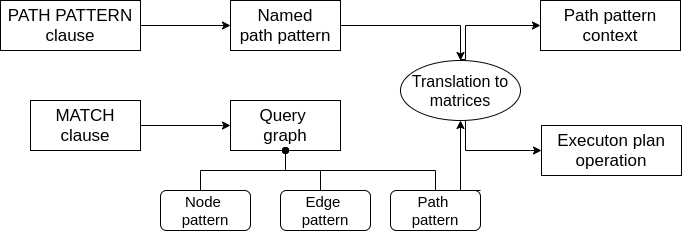
\includegraphics[width=\linewidth]{execution-plan-building.png}
  \caption{Extension diagram for building a query execution plan}
\end{figure}

In the RedisGraph the main part of processing a query is building its execution plan. Execution plan consists of operations that perform basic processing such as filtering, pattern matching, aggregation and result construction. Operations have parent-child relationships, so they are formed into a tree. Each operation can consume a record from a child operation, process it and produce another one for the parent. Records contain information necessary for the parent operation, as well as everything to restore the response, such as identifiers of accumulated vertices and edges.

Path patterns relates to the pattern matching operations and is very similar to relationship patterns from the original Cypher. All pattern matching operations are derived from the MATCH clause that consists of relationship patterns and node patterns. In the first stage of processing, these patterns turn into an intermediate representation -- the \textit{query graph}. The nodes and edges of the \textit{query graph} corresponds to node and relationship patterns. We extended query graph to be able to contain path patterns. Thus the query graph edges can be either relationship or path patterns, which are stored in a more convenient intermediate representation other than AST.

At the second stage, the query graph is translated into algebraic expressions over matrices. To do this, RedisGraph first linearizes the query graph, and then splits it into small paths. After that, each path is translated into a single algebraic expression. Its operands are a matrices specifying the type of edges and labels of vertices. To support path patterns we first extended the split processing so that each path template corresponds to exactly one path after query graph splitting. After that we implemented translation of the path patterns into an algebraic expressions. To do this we needed to extend the matrix operands to support references to named paths patterns in algebraic expressions. Finally we have developed the semantics of path patterns in terms of algebraic expressions over matrices.

In the last stage execution plan operations are built and appended to execution plan. Each operation derived from single algebraic expression. The extension of the execution plan operation related to path patterns is described in \autoref{subsubsec:execution-plan-evaluating}.

Other processing that occurs during the execution plan construction and was supported by us is related to named path patterns. They are processed independently of the unnamed path patterns found in MATCH clause and don't produce execution plan operations. All named path patterns are collected from \lstinline{PATH PATTERN} clauses. Then they translated into algebraic expressions and stored in the corresponding global context of the query -- \textit{path pattern context}. It is used in initializing the operations of the execution plan, which is described in~\autoref{subsubsec:execution-plan-evaluating}.

\subsubsection{Execution plan evaluating}
\label{subsubsec:execution-plan-evaluating}
% CFPQ to matrix expressions, etc. General schema of integration. Limits, restrictions, examples, etc.

\subsection{Evaluation}

Small basic evalustion on real-world graph (geo?).
In order to show, that performance is reasonable.

Regular quries. Comparison with other DB?

